
%\input{stat-sinica-header.tex}

\documentclass[12pt]{article}\usepackage[]{graphicx}\usepackage[]{xcolor}
% maxwidth is the original width if it is less than linewidth
% otherwise use linewidth (to make sure the graphics do not exceed the margin)
\makeatletter
\def\maxwidth{ %
  \ifdim\Gin@nat@width>\linewidth
    \linewidth
  \else
    \Gin@nat@width
  \fi
}
\makeatother

\definecolor{fgcolor}{rgb}{0.345, 0.345, 0.345}
\newcommand{\hlnum}[1]{\textcolor[rgb]{0.686,0.059,0.569}{#1}}%
\newcommand{\hlstr}[1]{\textcolor[rgb]{0.192,0.494,0.8}{#1}}%
\newcommand{\hlcom}[1]{\textcolor[rgb]{0.678,0.584,0.686}{\textit{#1}}}%
\newcommand{\hlopt}[1]{\textcolor[rgb]{0,0,0}{#1}}%
\newcommand{\hlstd}[1]{\textcolor[rgb]{0.345,0.345,0.345}{#1}}%
\newcommand{\hlkwa}[1]{\textcolor[rgb]{0.161,0.373,0.58}{\textbf{#1}}}%
\newcommand{\hlkwb}[1]{\textcolor[rgb]{0.69,0.353,0.396}{#1}}%
\newcommand{\hlkwc}[1]{\textcolor[rgb]{0.333,0.667,0.333}{#1}}%
\newcommand{\hlkwd}[1]{\textcolor[rgb]{0.737,0.353,0.396}{\textbf{#1}}}%
\let\hlipl\hlkwb

\usepackage{framed}
\makeatletter
\newenvironment{kframe}{%
 \def\at@end@of@kframe{}%
 \ifinner\ifhmode%
  \def\at@end@of@kframe{\end{minipage}}%
  \begin{minipage}{\columnwidth}%
 \fi\fi%
 \def\FrameCommand##1{\hskip\@totalleftmargin \hskip-\fboxsep
 \colorbox{shadecolor}{##1}\hskip-\fboxsep
     % There is no \\@totalrightmargin, so:
     \hskip-\linewidth \hskip-\@totalleftmargin \hskip\columnwidth}%
 \MakeFramed {\advance\hsize-\width
   \@totalleftmargin\z@ \linewidth\hsize
   \@setminipage}}%
 {\par\unskip\endMakeFramed%
 \at@end@of@kframe}
\makeatother

\definecolor{shadecolor}{rgb}{.97, .97, .97}
\definecolor{messagecolor}{rgb}{0, 0, 0}
\definecolor{warningcolor}{rgb}{1, 0, 1}
\definecolor{errorcolor}{rgb}{1, 0, 0}
\newenvironment{knitrout}{}{} % an empty environment to be redefined in TeX

\usepackage{alltt}

\setlength{\abovecaptionskip}{-2mm}

%%%%%%% START OF STAT SINICA SETTINGS %%%%%%%%%%

\textwidth=31.9pc
\textheight=46.5pc
\oddsidemargin=1pc
\evensidemargin=1pc
\headsep=15pt
\topmargin=.6cm
\parindent=1.7pc
\parskip=0pt

\usepackage[sectionbib]{natbib}
\usepackage{array,epsfig,fancyheadings,rotating}
%\usepackage[]{hyperref}  %<----modified by Ivan
%%%%%%%%%%%%%%%%%%%%%%%%%%%%%%%%%%%%
\usepackage{sectsty, secdot}
\sectionfont{\fontsize{12}{15}\selectfont}
\sectionfont{\fontsize{12}{14pt plus.8pt minus .6pt}\selectfont}
\renewcommand{\theequation}{\thesection\arabic{equation}}
\subsectionfont{\fontsize{12}{14pt plus.8pt minus .6pt}\selectfont}
%%%%%%%%%%%%%%%%%%%%%%%%%%%%%%%%%%%%%%%%%%%%%%%%%%%%%%%%%%%%%%%%%%%%%%%%%%%%%%

\pagestyle{fancy}
\def\n{\noindent}
\lhead[\fancyplain{} \leftmark]{}
\chead[]{}
\rhead[]{\fancyplain{}\rightmark}
\cfoot{}

%%%%%% END OF STAT SINICA SETTINGS %%%%%%%%5

% sec:intro.
% sec:alg. The \code{ibpf} algorithm for likelihood maximization
% sec:sim. Testing ibpf on a measles transmission model: simulation results
% sec:model. (subsection) The measles data and model
% sec:data. Data analysis results
% sec:discussion.



\newcommand\jwc[1]{\textcolor{orange}{[#1]}}

\newcommand\mytitle{An iterated block particle filter for inference on coupled dynamic systems with shared and unit-specific parameters}

\newcommand\ibpf{IBPF}

\newcommand\supSecMeaslesParams{S1}
\newcommand\supSecAlg{S2}
\newcommand\supSecEfficiency{S3}
\newcommand\supFigSpatReg{S1}

%\usepackage[sectionbib]{natbib}

%% for algorithm pseudocode
\usepackage{enumerate,alltt,xstring}
\usepackage[ruled,noline,linesnumbered]{algorithm2e}
\usepackage{setspace}
\SetKwFor{For}{for}{do}{end}
\SetKwFor{While}{while}{do}{end}
\SetKwInput{KwIn}{input}
\SetKwInput{KwOut}{output}
\SetKwInput{KwCplx}{complexity}
\SetKwInput{KwIndices}{note}
\SetKwBlock{Begin}{procedure}{}
\DontPrintSemicolon

% for measles model
\newcommand\amplitude{h}
\newcommand\meanBeta{{\overline\beta}}
\newcommand\cohort{c}
\newcommand\birth{b}
\newcommand\gravity{G}
%\newcommand\pop{p}  % average population over time
\newcommand\pop{\mathrm{pop}}  % average population over time
\newcommand\schoolTermFrac{s}
\newcommand\pinit{\pi}
\newcommand\birthdelay{\Delta}

%%%%%%%%%%%%%%%% START OF USER DEFINITIONS %%%%%%%%%%%%%%%5

\newcommand\siOnly[1]{} %% redefined for the supplement
\newcommand\msOnly[1]{#1} %% redefined for the supplement

%% code macros
%\newcommand\slot[1]{\code{#1}}
\newcommand\class[1]{class `\code{#1}'}
\newcommand\code[1]{\texttt{#1}}
\usepackage{url}
\newcommand\spatPomp{\texttt{spatPomp}}

%% EDITING MACROS

%\usepackage[normalem]{ulem}% to use \sout in feedback commands
%\usepackage{subfigure,sidecap}
%\usepackage{wrapfig}
\usepackage{color}
\usepackage[normalem]{ulem}% to use \sout in feedback commands
% orange for EI
\definecolor{orange}{rgb}{1,0.5,0}
\newcommand\ei[2]{\sout{#1} \textcolor{orange}{#2}}
\newcommand\eic[1]{\textcolor{orange}{[#1]}}
% green for KA
\definecolor{green}{rgb}{0,0.5,0}
\newcommand\ka[2]{\sout{#1} \textcolor{green}{#2}}
\newcommand\kac[1]{\textcolor{green}{[#1]}}
%purple for AK
%\definecolor{purple}{rgb}{0.5,0,1}
%\newcommand\ak[2]{\sout{#1} \textcolor{purple}{#2}}
%\newcommand\akc[1]{\textcolor{purple}{[#1]}}
%cyan for JP
\definecolor{cyan}{rgb}{0,.5,.5}
\newcommand\jp[2]{\sout{#1} \textcolor{cyan}{#2}}
\newcommand\jpc[1]{\textcolor{cyan}{[#1]}}

%% basic POMP definitions
\newcommand\Xspace{{\mathbb X}}
\newcommand\Yspace{{\mathbb Y}}
%\newcommand\Thetaspace{{\Theta}}
\newcommand\Thetaspace{\R^{\Thetadim}}
\newcommand\Xunitspace{{\scriptsize{\mathcal X}}}
\newcommand\Yunitspace{{\tiny{\mathcal Y}}}
\newcommand\hatTheta{\widehat{\Theta}}
\newcommand\Xdim{{\mathrm{dim}}(\Xspace)}
\newcommand\Ydim{{\mathrm{dim}}(\Yspace)}
%\newcommand\Thetadim{{\mathrm{dim}}(\Thetaspace)}
\newcommand\Thetadim{P}
\newcommand\thetadim{p}
\newcommand\timeSet{{\mathbb T}}
\newcommand\data[1]{#1^*}

\newcommand\unitSpecific{\hspace{0.1mm}\mathrm{us}}
\newcommand\shared{\hspace{0.15mm}\mathrm{sh}}

\newcommand\comma{{\hspace{-0.25mm},\hspace{-0.2mm}}}

%% for measles model

%\newcommand\modelA{(A)}
%\newcommand\modelB{(B)}
%\newcommand\modelC{(C)}
\usepackage[mathscr]{euscript}
\newcommand\modelA{$\mathscr{A}$}
\newcommand\modelB{$\mathscr{B}$}
\newcommand\modelC{$\mathscr{C}$}
\newcommand\measOD{\tau}

%% for particle filters
\newcommand\unit{u}
\newcommand\altUnit{\tilde u}
\newcommand\Unit{U}
\newcommand\rep{i}
\newcommand\Rep{\mathcal{I}}
\newcommand\island{\rep}
\newcommand\Island{\Rep}
%\newcommand\txtisland{replicate}
\newcommand\altIsland{\tilde i}
\usepackage[mathscr]{euscript}

\renewcommand\time{n}
\newcommand\myvec[1]{\boldsymbol{#1}}
\newcommand\altTime{\tilde n}
\newcommand\Time{N}
\newcommand\Np{J}
\newcommand\np{j}
\newcommand\altNp{k}
\newcommand\altAltNp{\tilde j}
\newcommand\resampleIndex{i}
\newcommand\unitWeight{w}
\newcommand\spatReg{r}


%% for all iterated filtering algorithms
\newcommand\Nit{M}
\newcommand\nit{m}

%% for Bpfilter
\newcommand\block{k}
\newcommand\Block{K}
\newcommand\blockweight{w}
\newcommand\blocklist{\mathcal{B}} %% Partition

%% customized math macros
\newcommand\prob{\mathbb{P}}
\newcommand\E{\mathbb{E}}
\newcommand\dd[1]{\mathrm{d}{#1}}
\newcommand\given{{\,\vert\,}}
\newcommand\equals{{{\,}={\,}}}
\newcommand\myequals{\hspace{0.5mm}{=}\hspace{0.5mm}}
\newcommand\myto{{\;:\;}}
\newcommand\mycolon{{\hspace{0.6mm}:\hspace{0.6mm}}}
\newcommand\seq[2]{{#1}\mycolon{#2}}
\newcommand\mydot{{\,\cdot\,}}
\newcommand\cp[2]{N_{\mathrm{#1}\mathrm{#2}}}
\newcommand\giventh{{\hspace{0.5mm};\hspace{0.5mm}}}
%\newcommand\normal{{\mathrm{Normal}}}
\newcommand\normal{\mathcal{N}}
\newcommand\argequals{{\,=\,}}
\newcommand\lags{c}
\newcommand\maxlag{\overline{c}}
\newcommand\nlfList{C}
\newcommand\bigO{\mathcal{O}}
\newcommand\loglik{\lambda}
\newcommand\loglikMC{\MC{\loglik}}
\newcommand\R{\mathbb{R}}
\newcommand\param{\,;}
\newcommand\MC[1]{#1^{\,\mbox{\tiny MC}}}
\newcommand\EMC{{\E}}
\newcommand\Var{\mathrm{Var}}
\newcommand\var{\Var}
\newcommand\Cov{\mathrm{Cov}}
\newcommand\cov{\Cov}
\newcommand\iid{\mathrm{iid}}
%\newcommand\dist{\mathrm{dist}}
\newcommand\dist{d}
\newcommand\transpose{\top}

\def\lik{L}
\def\loglik{\ell}

%% THEOREM-LIKE ENVIRONMENTS
\usepackage{amsthm}
\newtheorem{prop}{Proposition}
\newtheorem{theorem}{Theorem}
\newtheorem{lemma}{Lemma}
\newtheorem{example}{Example}
\newtheorem{remark}{Remark}
\newtheorem{cor}{Corrolary}
\newtheorem{fact}{Fact}
\newtheorem{assumption}{Assumption}
\newtheorem{assumptionB}{Assumption}
%\newtheorem{procedure}{Procedure}
\renewcommand\theassumption{A\arabic{assumption}}
\renewcommand\theassumptionB{B\arabic{assumptionB}}

%\usepackage{float}
%\floatstyle{ruled}
%\newfloat{textbox}{t}{tbx}
%\floatname{textbox}{Box}
%\renewcommand\thetextbox{\arabic{textbox}}



%%%%%%%%%%%%%%%% END OF USER DEFINITIONSS %%%%%%%%%%%%%%%5


\usepackage{amsmath,amssymb}
%\usepackage{graphicx,psfrag,epsf}
\usepackage{graphicx}
\usepackage{enumerate}
\usepackage{natbib}
\usepackage{soul}
\usepackage{xcolor}

\usepackage{url} % not crucial - just used below for the URL 

%\newcommand\jpc[1]{{\textcolor{orange}{#1}}}
\newcommand\aak[1]{{\textcolor{blue}{#1}}}

%\usepackage{fullpage}
\bibliographystyle{apalike}








% \date{This manuscript was compiled on \today}
\IfFileExists{upquote.sty}{\usepackage{upquote}}{}
\begin{document}

%%%%%%%%%%%%%%%%%%%%%%%%%%%%%%%%%%%%%%%%%%%%%%%%%%%%%%%%%%%%%%%%%%%%%%%%%%%%%%%%%%%%%%%%%%%%%%%%%%%%%%%%%%%%%%%%%%%%%%%%%%%%
%%%%%%%%%%%%%%%%%%%%%%%%%%%%%%%%%%%%%%%%%%%%%%%%%%%%%%%%%%%%%%%%%%%%%%%%%%%%%%%%%%%%%%%%%%%%%%%%%%%%%%%%%%%%%%%%%%%%%%%%%%%%

\renewcommand{\baselinestretch}{1.5}

\markright{ \hbox{\footnotesize\rm Statistica Sinica
%{\footnotesize\bf 24} (201?), 000-000
}\hfill\\[-13pt]
\hbox{\footnotesize\rm
%\href{http://dx.doi.org/10.5705/ss.20??.???}{doi:http://dx.doi.org/10.5705/ss.20??.???}
}\hfill }

\markboth{\hfill{\footnotesize\rm E. L. Ionides et al.} \hfill}
{\hfill {\footnotesize\rm An iterated block particle filter} \hfill}

\renewcommand{\thefootnote}{}
$\ $\par

%%%%%%%%%%%%%%%%%%%%%%%%%%%%%%%%%%%%%%%%%%%%%%%%%%%%%%%%%%%%%%%%%%%%%%%%%%%%%%%%%%%%%%%%%%%%%%%%%%%%%%%%%%%%%%%%%%%%%%%%%%%%

\fontsize{12}{14pt plus.8pt minus .6pt}\selectfont \vspace{0.8pc}
\centerline{\large\bf An iterated block particle filter for inference on coupled dynamic}
\vspace{2pt} 
\centerline{\large\bf systems with shared and unit-specific parameters}
\vspace{.4cm} 
\centerline{E. L. Ionides, J. Wheeler and N. Ning}
\vspace{.4cm} 
\centerline{University of Michigan, department of Statistics,}

 \vspace{.55cm} \fontsize{9}{11.5pt plus.8pt minus.6pt}\selectfont


\centerline{Submitted to {\it Statistica Sinica} special edition on}
\centerline{Recent developments of sequential Monte Carlo methods}
\centerline{and their applications}


%%%%%%%%%%%%%%%%%%%%%%%%%%%%%%%%%%%%%%%%%%%%%%%%%%%%%%%%%%%%%%%%%%%%%%%%%%%%%%%%%%%%%%%%%%%%%%%%%%%%%%%%%%%%%%%%%%%%%%%%%%%%

\begin{quotation}
\noindent {\it Abstract:}
We consider inference for a collection of partially observed, stochastic, interacting, nonlinear dynamic processes.
Each process is identified with a label called its unit, and our primary motivation arises in biological metapopulation systems where a unit corresponds to a spatially distinct sub-population.
Metapopulation systems are characterized by strong dependence through time within a single unit and relatively weak interactions between units, and these properties make block particle filters an effective tool for simulation-based likelihood evaluation. 
Iterated filtering algorithms can facilitate likelihood maximization for simulation-based filters.
We introduce a new iterated block particle filter algorithm applicable when parameters are unit-specific or shared between units.
We demonstrate this algorithm by performing inference on a coupled epidemiological model describing spatiotemporal measles case report data for twenty towns.

\vspace{9pt}
\noindent {\it Key words and phrases:}
sequential Monte Carlo; metapopulation; spatiotemporal; maximum likelihood estimation; partially observed Markov process.
\par
\end{quotation}\par



\def\thefigure{\arabic{figure}}
\def\thetable{\arabic{table}}

\renewcommand{\theequation}{\thesection.\arabic{equation}}


\fontsize{12}{14pt plus.8pt minus .6pt}\selectfont


%% \def\spacingset#1{\renewcommand{\baselinestretch}%
%% {#1}\small\normalsize} \spacingset{1}


\date{}

%% \spacingset{1.45} 

\section{Introduction}
\label{sec:intro}


Statistical inference for high-dimensional partially-observed nonlinear dynamic systems arises in various scientific contexts.
Massive models and datasets are considered in the geophysical sciences, carried out under the name of data assimilation \citep{evensen09book}.
Population models in ecology and epidemiology can be characterized by high levels of stochasticity, nonlinearity, measurement error, and model uncertainty, leading to challenges of a somewhat different nature than geophysical models.
In addition, biological population systems may sometimes have low population due to local introductions or fade-outs of one or more constituent species.
Low population situations may require consideration of integer-valued counts rather than continuous population approximations.
Collections of biological populations measured at different spatial locations may have spatial interactions in addition to local population dynamics; such collections are called a metapopulation.
The study of spatiotemporal disease dynamics has motivated research into inference for metapopulation systems \citep{xia04,li20,park20,ionides21,cauchemez08,bjornstad19}.

Statistical inference for partially observed nonlinear biological systems was an open methodological challenge until recently even in the time series case \citep{bjornstad01}.
Advances in Monte Carlo methods based on the particle filter have made inference accessible on many low-dimensional problems, but the curse of dimensionality \citep{bengtsson08} prevents applicability of the basic particle filter on metapopulations with more than a few units.
Methods based on improving the proposal distribution for the particle filter may not fully resolve the curse of dimensionality \citep{snyder15}.
Situations where previous Monte Carlo methods can provably beat the curse of dimensionality may have limited applicability \citep{beskos17,park20,ionides21}.
Consequently, state-of-the-art analysis has depended on ensemble Kalman filter (EnKF) methods \citep{li20}.
EnKF algorithms scale well but are founded on an approximation that can be unsuitable for discrete populations with fade-out and re-introduction dynamics and other highly non-Gaussian features \citep{ionides21}.

In Sec.~\ref{sec:alg}, we propose an algorithm for inference on metapopulation dynamics which we call an iterated block particle filter (IBPF).
IBPF extends the block particle filter (BPF) of \citet{rebeschini15} to carry out maximum likelihood parameter estimation.
A previous IBPF algorithm was developed by \citet{ning21-ibpf} for the particular case that all estimated parameters are unit-specific, which is to say that the dynamics and measurement process for a unit $u$ are determined by a set of parameters $\psi_u$ specific to unit $u$.
The formal meaning of this assertion is given, together with the pseudocode for our algorithm, in Sec.~\ref{sec:alg}.
We propose an extension of their IBPF which additionally permits the estimation of a vector of shared parameters, $\phi$.
In this case, the full parameter vector is $\theta=(\phi,\psi_{1:U})$ where the $U$ units are labeled $\{1,\dots,\Unit\}$ which we denote by $\seq{1}{\Unit}$.
\citet{ning21-ibpf} developed theoretical justification for their algorithm, but our extension of IBPF currently carries only empirical support.

There may be scientific interest concerning which parameters in metapopulation systems are best understood as unit-specific, and which can reasonably be modeled as shared between units.
Another relevant possibility is that a parameter may differ between units as a shared function of unit-specific covariates, which formally is a special case of a shared parameter.
Addressing these issues is also prerequisite for studying questions about coupling of metapopulation systems via model-based inference from spatiotemporal data.
We will show empirically, in Sec.~\ref{sec:data}, that our {\ibpf} algorithm is applicable to an inference challenge in epidemiological metapopulation dynamics.
Our demonstration focuses on a dataset for weekly measles incidence in 20 towns in the United Kingdom (UK) during the pre-vaccination era \citep{he10} modeled using a previously studied metapopulation model \citep{park20,ionides21}.
Measles case reports have been a longstanding benchmark problem for inference on biological dynamics, motivating the development of time series methodology and, more recently, the progression from single populations to metapopulation systems.
Unlike previous attempts on sequential Monte Carlo inference for metapopulation models, we show that our algorithm can provide practical inference when parameters are either shared between units or differ between units.
Our data analysis results do not fully resolve open questions about what models for coupling between towns are supported by the data, and which parameters should be modeled as unit-specific.
Rather, we demonstrate steps toward this research goal.
We use a simulation study, in Sec.~\ref{sec:sim}, to show that our methodology can deliver a good approximation to the maximum likelihood estimate when fitting the model used to simulate the data.
This reassurance allows us to interpret our data analysis results as evidence of model misspecification, providing a guide for future investigations of these data as well as tools to carry out those investigations.

Optimization of high-dimensional, non-convex and potentially multi-modal functions, evaluated using stochastic methods, is not straightforward even when it is possible to evaluate the function within an acceptable level of error.
Therefore, we discuss approaches that assist the noisy likelihood searches, and suggest diagnostic plots to assess their success.

\section{The {\ibpf} algorithm for likelihood maximization}
\label{sec:alg}

A latent Markov process is denoted by $\{\myvec{X}_{\time},\time\in \seq{0}{\Time}\}$, with $\myvec{X}_{\time}=X_{1:\Unit,\time}$ taking values in a product space $\Xspace^\Unit$.
We define set-valued subscripts by $X_A=\{X_a,a\in A\}$ and $X_{A,B}=\{X_{a,b}, a\in A, b\in B\}$.
The discrete time process $\myvec{X}_{0:\Time}$ may arise from a continuous time Markov process $\{\myvec{X}(t), t_0\le t\le t_{\Time} \}$ observed at times $t_{1:\Time}$, and in this case we set $\myvec{X}_\time=\myvec{X}(t_\time)$.
The initial value $\myvec{X}_{0}$ may be stochastic or deterministic.
Observations are made on each unit, modeled by an observable process $\myvec{Y}_{1:\Time}=Y_{1:\Unit,1:\Time}$ which takes values  at each time $\time$ in a product space $\Yspace^\Unit$.
Observations are modeled as conditionally independent given the latent process.
The conditional independence of measurements applies over both time and the unit structure, so the collection $\big\{Y_{\unit\comma\time},\unit\in\seq{1}{\Unit},\time\in\seq{1}{\Time}\big\}$ is conditionally independent given
$\big\{X_{\unit\comma\time},\unit\in\seq{1}{\Unit},\time\in\seq{1}{\Time}\big\}$.
We suppose the existence of a joint density $f_{\myvec{X}_{0:\Time},\myvec{Y}_{1:\Time}}$  for $X_{1:\Unit,0:\Time}$ and $Y_{1:\Unit,1:\Time}$ with respect to some appropriate measure, following a notational convention that the subscripts of $f$ denote the joint or conditional density under consideration.
We suppose that $f$ depends on a parameter vector $\theta=(\phi,\psi_{1:U})$.
The data are $\data{y}_{\unit\comma\time}$ for unit $\unit$ at time $\time$.
This model is a special case of a  partially observed Markov process (POMP) also known as a state space model or hidden Markov model.
The additional unit structure, not generally required for a POMP, is appropriate for modeling interactions between units characterized by a spatial location, and so we call the model a SpatPOMP.
For metapopulation models, the units are not generally arranged on a spatial grid but comprise a collection of spatially distributed population centers.

A numerical challenge of fundamental statistical relevance is the maximization of the log-likelihood function of the data given the model, $\loglik(\theta)=\log f_{\myvec{Y}_{1:\Time}}(\data{\myvec{y}}_{1:\Time}\giventh \theta)$.
Numerical evaluation of the likelihood function is closely related to the filtering problem of evaluating $f_{\myvec{X}_n|\myvec{Y}_{1:n}}(\myvec{x}_n\given \data{\myvec{y}}_{1:n}\giventh \theta)$.
Including parameters into the latent space of a dynamic model can coerce a filter into calculating a Bayesian posterior distribution, though regularization is required to make the calculation numerically tractable using Monte Carlo methods \citep{kitagawa98,janeliu01}.
Iterating this Bayesian calculation recursively targets a maximum likelihood estimate (MLE), a strategy known as data cloning \citep{lele07,lele10}.
Adding noise to perturb the parameters at each time point can stabilize the numerics while retaining the capability to approximate the MLE \citep{ionides06-pnas,ionides11,ionides15}.
Many variations on this idea have been developed using different filter methods \citep{park20,li20,ionides21,manoli15} or employing different perturbation systems \citep{doucet13,nguyen17}.

Previous approaches to iterated perturbed particle filtering are not immediately applicable to BPF.
In the special case where each parameter is localized to an individual unit (i.e., all parameters are unit-specific) one can resample perturbed parameters at the block level and obtain a theoretical guarantee of approximating the MLE \citep{ning21-ibpf}.
Formally, we say that a parameter for a discrete-time SpatPOMP is specific to a unit $u$ if it is involved in specifying the measurement density $f_{Y_{u,n}|X_{u,n}}$ or transition density $f_{X_{u,n+1}|\myvec{X}_n}$ for some $n$, and it is not involved in $f_{Y_{v,m}|X_{v,m}}$ or $f_{X_{v,m+1}|\myvec{X}_m}$ for any $v\neq u$ and any $m$.
For a continuous-time SpatPOMP, we replace the requirement on $f_{X_{u,n+1}|\myvec{X}_n}$ with an equivalent requirement on a numerical solution over a small time increment $\delta$, as in equation \eqref{eq:extension} below.
A parameter which is not unit-specific is said to be shared between units.
There are intermediate possibilities, where a parameter shared for only a subset of all units, but such situations are not explored further here.
The special case where all parameters are unit-specific may arise sometimes, but models typically have some shared parameters which arise in transition densities and/or measurement densities for multiple units. 

Our approach to iterated filtering for shared parameters involves constructing an extended model within which the a shared parameters is represented as a unit-specific parameter that happens to be constant across units.
We construct a spatiotemporally extended model by supposing a numerical solution for the transition from time $t$ to time $t+\delta$ for each unit $u$ with the form
\begin{equation}
\label{eq:extension}
  X_{\unit}(t+\delta) = X_\unit(t) + Q_u(\myvec{X}(t),\myvec{\eta}_t,\phi,\psi_{\unit},t,\delta),
\end{equation}
where the random vector $\myvec{\eta}_t=\eta_{1:\Unit,t}$ is shared for all $u\in \seq{1}{U}$ and does not depend on $\theta$.
If a representation \ref{eq:extension} exists, an extended model is defined by replacing $\phi$ with $\phi_{\unit}(t)$ and $\psi_u$ with $\psi_{u}(t)$.
Equation \ref{eq:extension} implicitly defines a continuous-time extended model by the limit as $\delta\to 0$, when that limit exists, but for simulation-based methods the numerical solution is of more immediate concern than this limit.
Admitting a minor abuse of notation, we subsequently use a density $f$ to denote both the original model and its extension for spatiotemporally varying parameters, with the context determining which one is intended.


In some situations, the extended model could have problematic properties.
For example, it could break conservation laws obeyed by the original system.
In other situations, the extended model may make scientific sense in its own right.
For example, in biological metapopulation systems it might be scientifically meaningful to consider a model where there is variation over space and time in the parameters describing the local dynamics.
Here, we are focusing on the hypothesis that there are some parameters that are fixed across space and time, but the specification in \eqref{eq:extension} requires this hypothesis to be nested within a more flexible alternative.

The IBPF algorithm described in Alg.~\ref{alg:ibpfilter} carries out a block particle filter on this extended model.
The extended parameters are given independent perturbations, but a spatial autoregressive step pulls the values of shared parameters toward their mean over the units.
Indeed, this autoregressive step is the only difference between  Alg.~\ref{alg:ibpfilter} and the algorithm for unit-specific parameters proposed by \citet{ning21-ibpf}.
This algorithm, in turn, is essentially the IF2 algorithm of \citet{ionides15} with the particle filter replaced by BPF.
Alg.~\ref{alg:ibpfilter} assumes implicit loops over $\np\ \text{in}\ \seq{1}{\Np}$ and $\unit\ \text{in}\ \seq{1}{\Unit}$, 
$\normal(\mu,\Sigma)$ denotes the normal distribution with mean $\mu$ and variance matrix $\Sigma$, and
$\sigma_\time$ is a $D\times D$ diagonal matrix with entries $\sigma_{d,\time}$.

The pseudocode in Alg.~\ref{alg:ibpfilter} represents our implementation of {\ibpf} as the R function \code{ibpf} in the open-source package \code{spatPomp} \citep{asfaw21github,asfaw21arxiv}.
We will contribute \code{ibpf} to \code{spatPomp}.
Aadditionally, the source code for all the results in this article is available at \url{https://github.com:ionides/ibpf_article}.
Various generalizations of this implementation are possible.
For example, iterated filtering theory does not rely on parameter perturbations following the normal distribution \citep{ionides15} though in practice we transform parameters to facilitate this convenient choice.
Also, the pseudocode does not include parameter-dependent random walk variance, or a different perturbation schedule for initial value parameters, both of which could be included.

%%%%%%% ibpf BBBBBBBBBBBBBBBBBBBBBBBBBBBBBBBBB %%%%%%%%%%%%%%%%%


\begin{algorithm}[H]	
   \caption{\textbf{IBPF}. \\
    {\bf Inputs}:
   simulator for the extended model, $f_{\myvec{X}_{\time}|\myvec{X}_{\time-1}}(\myvec{x}_{\time}\given \myvec{x}_{\time-1}\giventh\myvec{\theta})$;
    evaluator for $f_{{Y}_{\unit,\time}|{X}_{\unit,\time}}({y}_{\unit,\time}\given {x}_{\unit,\time}\giventh\theta)$;
    simulator for extended initialization, $f_{\myvec{X}_0}(\myvec{x}_0\giventh\myvec{\theta})$;
    data, $\data{\myvec{y}}_{1:\Time}$;
    number of particles, $\Np$;    
    blocks, $\blocklist_{1:\Block}$;
    initial parameter swarm with decomposition into shared and unit-specific parameters, $\Theta^{0,\np}_{\unit}=(\Phi^{0,\np}_{\unit},\Psi^{0,\np}_{\unit})$;
    random walk perturbation, $\sigma_{d,\time}$.
%{\bf \code{spatPomp} implementation}:	
%     \code{ibpf(P,\,
%        params{\argequals}$\theta_0${\argequals}$(\phi_0,\psi_{1:\Unit,0})$,
%        Nbpf{\argequals}$\Nit$,
%        Np{\argequals}$\Np\!$,
%        rw.sd{\argequals}$\sigma$,
%        cooling.fraction.50{\argequals}$a$,
%        spat.regression{\argequals}$\spatReg$,
%        block\_list{\argequals}$\blocklist$\,)}	
%    where \code{P} is a	
%     \class{\spatPomp} object \citep{asfaw21arxiv}.
%
}\label{alg:ibpfilter}	
%\BlankLine	
\For{$\nit\ \mathrm{in}\ \seq{1}{\Nit}$}{	
  Perturb parameters:
    $\Theta^{F,\nit,\np}_{\unit,0}\sim \normal
    \left(
      \Theta^{\nit-1,\np}_{\unit}\param \sigma^2_{0} a^{2\nit/50}
    \right)$
  \;
  Initialization:  simulate $\myvec{X}_{0}^{F,\np}\sim {f}_{\myvec{X}_{0}}
    \left(\mydot\giventh{\Theta^{F,\nit,\np}_{1:\Unit,0}}\right)$\;
    \For{$\time\ \mathrm{in}\ \seq{1}{\Time}$}{ % For each time step
      Perturb parameters:
        $\Theta^{P,\nit,\np}_{\unit,\time}\sim \normal\left(
       \Theta^{F,\nit,\np}_{\unit,\time-1},\sigma^2_\time a^{2\nit/50} \right)$
     \;
      Prediction simulation: $\myvec{X}_{\time}^{P,\np}
        \sim {f}_{\myvec{X}_{\time}|\myvec{X}_{\time-1}}\big(
        \mydot|\myvec{X}_{\time-1}^{F,\np};{\Theta^{P,\nit,\np}_{1:\Unit,\time}}\big)$	
      \;	
    \For{$\block\ \mathrm{in}\ \seq{1}{\Block}$}{
      Block prediction weights:
            $\displaystyle \blockweight^P_{\time,\np, \block}=
              \prod_{\unit \in \blocklist_{\block}}
              f_{Y_{\unit,\time}|X_{\unit,\time}}
              \big(
              \data{y}_{\unit,\time}\given X^{P,\np}_{\unit,\time}
                \giventh \Theta^{P,\nit,\np}_{\unit,\time} \big)$	
            \nllabel{alg:bpfilter:blockweights}
      \;
      Normalize weights:
        $\tilde{\blockweight}_{\time,\np, \block}= \blockweight^P_{\time,\np,\block}\Big/
        \sum_{i=1}^{\Np}\blockweight^P_{\time,i,\block}$\;
      Select resample indices:
        $\resampleIndex_{1:\Np,\block}$ with
        $\prob\left[\resampleIndex_{\np,\block}=\altNp\right] =
        \tilde{\blockweight}_{\time,\np,\block}$
      \;
         $X_{\blocklist_{\block},\time}^{F,\np}=X_{\blocklist_{\block},\time}^{P,\resampleIndex_{\np,\block}}$,
	$\Theta_{\blocklist_{\block},\time}^{F,\np}
	  =\Theta_{\blocklist_{\block},\time}^{P,\resampleIndex_{\np,\block}}
	  =\big(\Phi_{\blocklist_{\block},\time}^{P,\resampleIndex_{\np,\block}},
	    \Psi_{\blocklist_{\block},\time}^{P,\resampleIndex_{\np,\block}}\big)$
         \nllabel{alg:bpfilter:resample}
      \;
      block mean of shared parameters: $\mu_{\block,\time}^{} = \Np^{-1}\sum_{\np=1}^{\Np} \Phi^{F,\np}_{\blocklist_{\block},\time}$
    } %End of for loop over blocks
    overall mean of shared parameters: $\mu_{\time}^{} = \Block^{-1}\sum_{\block=1}^{\Block} \mu_{\block,\time}^{}$
    \;
    autoregressive correction:
    $\Phi^{F,\np}_{\blocklist_{\block},\time} = \Phi^{F,\np}_{\blocklist_{\block},\time} + \spatReg\big( \mu_{\time}^{} - \mu_{\block,\time}^{}  \big)$
  \;
  }%End timestep for Loop
  $\Theta_{\unit}^{\nit,\np}=\Theta^{F,\nit,\np}_{\unit,\Time}$
  \;  
} % end iterated filtering loop
\KwOut{	
    IBPF parameter swarm, $\Theta_{\unit}^{\Nit,\np}$
}	
\end{algorithm}	






\subsection{Algorithmic parameters}

Model parameters are optimized on a transformed scale for which unit variation is scientifically meaningful.
In practice, this means working with positive parameters on a log scale, and $(0,1)$ interval-valued parameters on a logistic scale.
We follow standard iterated filtering practice by using independent random walks for each parameter on this transformed scale \citep{king16}.
We discovered that the large number of parameters following a random walk, in the presence of unit-specific parameters, can require considerably smaller random walk standard deviations than the values around $\sigma_{d,n}=0.02$ (i.e., 2\% perturbation per time point) that have been employed for iterated filtering of time series models.
After experimentation, we used $\sigma_{d,n}=0.005$ for the initial search and $\sigma_{d,n}=0.00125$ for subsequent refinements.
Occasionally, a parameter which can be estimated precisely from the data can benefit substantially from a smaller perturbation.
This is the case for one parameter in our measles analysis, an exponent $\alpha$ for which the scale of uncertainty is an order of magnitude smaller than other parameters; therefore, $\sigma_{d,n}$ for this parameter was scaled accordingly.
In principle, $\sigma_{d,n}$ can be a function of $n$ as well as the parameter, $d$.
The most common reason for using this flexibility is to avoid perturbing parameters during time intervals when there is no information about them: following an evolutionary analogy, evolution cannot operate effectively when there is mutation but no selection.
For an initial value parameter, meaning one which specifies only the latent process value at the initial time $t_0$, we use $\sigma_{d,n}=0$ for $n\ge 1$ and we doubled the value of $\sigma_{d,n}$ for $n=0$.

We set the cooling rate parameter to be $a=0.5$, corresponding to a 1\% reduction in the random walk standard deviation at each iteration.
The only additional algorithmic parameter over previous iterated filtering algorithms is the spatial autoregressive parameter, $\spatReg$.
Numerical experimentation suggests that the performance is not sensitive to the choice of $\spatReg>0$ (see Fig~\ref{fig:spatreg_boxplot} in Appendix A).
Subsequently, we used $\spatReg=0.1$.

Applying IBPF to real data forces us to address issues of model development, model misspecification, and performance in the presence of outliers.
Before tackling these issues, we use simulated data to demonstrate the capabilities of the methodology on a correctly specified model.

\section{Testing {\ibpf} on a measles transmission model: simulation results}
\label{sec:sim}

Measles transmission has provided a useful example of epidemiological dynamics (and therefore also ecological dynamics, for a host-pathogen ecosystem), with plentiful case report data and relatively simple biology.
Model-based analysis of measles time series data led to advances in understanding of the seasonality of infectious disease \citep{fine82}, critical community size \citep{bartlett57}, the recognition that relatively simple mechanistic models can provide a remarkably good description of the dynamics \citep{earn00}, and much other foundational research on disease dynamics.
Some progress has been on building and fitting spatiotemporal models for measles; e.g., \citet{xia04,eggo11,bjornstad19,becker20}.
However, the lack of suitable methodology to fit and assess a flexible class of coupled models is an obstacle to further progress \citep{becker20}.
Previous methodological work has used spatiotemporal measles models as a test problem \citep{park20,ionides21}.
However, these methods have fallen short as tools for data analysis due to numerical considerations.
Bearing all this in mind, measles provides a natural testing ground for our new methodologies.
We demonstrate that we now have the tools to carry out likelihood maximization and profile likelihood confidence interval construction on mechanistic statistical models that are appropriate for spatiotemporal metapopulation disease data.

We specifically set ourselves the task of fitting a spatiotemporal model to the case reports for 20 towns studied by \citet{he10}.
We require ability to handle discrete case counts which vary from zero to thousands of cases per week.
We consider a model with the same structure as \citet{he10}, namely a Markov chain with Gamma noise on the infection rate, but with the addition of a term for transmission between cities.
This requirement limits us to plug-and-play methodologies, which are those that require simulation from the latent process model but not the ability to  evaluate transition densities \citep{breto09,he10}.
The model equations are given in Sec.~\ref{sec:model}.

\begin{knitrout}
\definecolor{shadecolor}{rgb}{1, 1, 1}\color{fgcolor}\begin{figure}

\includegraphics[width=6.5in]{figure/data-plot-1} \hfill{}

\caption[Weekly measles case reports for 20 UK towns]{Weekly measles case reports for 20 UK towns.}\label{fig:data-plot}
\end{figure}

\end{knitrout}

\begin{knitrout}
\definecolor{shadecolor}{rgb}{1, 1, 1}\color{fgcolor}\begin{figure}

\includegraphics[width=6.5in]{figure/sim-plot-1} \hfill{}

\caption[Simulated weekly measles case reports]{Simulated weekly measles case reports.}\label{fig:sim-plot}
\end{figure}

\end{knitrout}

The data are shown in Fig~\ref{fig:data-plot} and simulations from the model are shown in Fig~\ref{fig:sim-plot}.
Parameters for the simulated model were based on the analysis of individual towns by \citet{he10} and adjusted to provide a visual match in the simulations.
A goal of the simulation study is to obtain appropriate algorithmic choices for the data analysis, and to develop methodology which can be successful when the truth is known before applying it to data.
We present the simulation study from this perspective, to describe the process of developing our data analysis, though we acknowledge one could revisit the simulation study based on the data analysis in Sec.~\ref{sec:data} using maximum likelihood estimates of the parameters.

A key data analysis question is to decide which parameters should be shared between units and which should be unit-specific, taking distinct values on each unit.
For a general SpatPOMP parameter, it is not necessarily well-defined how to extend the model so that each unit has a distinct parameter value, however our measles model falls into the structure defined in \eqref{eq:extension} and we suspect that similar considerations may arise in other situations.
Different numerical issues may arise as the number of unit-specific parameters increases.
Each unit-specific parameter contributes $U$ dimensions to the parameter space, potentially contributing difficulties associated with high-dimensional or weakly identified parameters.
On the other hand, information about a unit-specific parameters may be localized in neighboring units which could align conveniently with the structure of the BPF.
Estimation of shared parameters, by contrast, has the task of harvesting information from across all the units, which may have its own difficulties.

Estimated parameter values may have scientific interest, but we focus on the statistical task of likelihood maximization.
In the presence of weak identifiability, small differences in likelihood could lead to large differences in parameter estimates.
In such sitatuations, a scientist may choose to investigate what functions of the parameters can be inferred accurately without adding additional assumptions, or alternatively they may choose to investigate the consequences of placing constraints on some parameters to improve identifiability of the remainder.
Likelihood maximization permits such investigations, but they are beyond the scope of this article.

To facilitate data analysis, we wish to have methodology that operates across the full spectrum of decisions on shared versus unit-specific parameter designations.
We therefore test our method on two cases: (A) mostly shared parameters, choosing only the initial values and reporting rate to be unit-specific; (B) every parameter is unit-specific.
We also consider a third case; (C) every parameter is unit-specific and the dynamic coupling (in our context, movement of infected individuals between towns) is replaced by an external forcing of each unit (in our context, an immigration rate of infected individuals from outside the study population).
Case (C) provides a useful point of reference since it is a special case of a PanelPOMP model \citep{breto19} and also can be analyzed as a collection of separate POMP models.
We set up our model so that in case (C) we retrieve the analysis of \citet{he10}.
One may expect that methods which take advantage of the special structure of (C) should out-perform more general methods that permit coupling between units, so we expect the SpatPOMP methods to be less numerically efficient than applying POMP methods separately to each unit.
Questions at stake are: How much less efficient are the SpatPOMP methods? Are simulation-based SpatPOMP inference methods practical for situations such as the measles model of \citet{he10}?


The simulated model is drawn from model (A), which is nested within model (B) but not within (C).
For models B and C, with all parameters are unit-specific, we must estimate $20\times 13=260$ parameters.
This greatly exceeds the 7 shared parameters fitted by \citet{ionides21} for a measles metapopulation model using a large computational effort.
An iterated guided intermediate resampling filter (IGIRF) algorithm was used to fit 9 shared parameters and 3 unit-specific initial value parameters in a measles metapopulation model \citep{park20}.
That analysis used a customized treatment for the unit-specific initial value parameters and did not attempt to estimate other unit-specific parameters.
IGIRF is sensitive to the choice of the guide function, and the model-specific implementation used by \citet{park20} performed better than the generic implementation of IGIRF currently available in \code{spatPomp}.
To our knowledge, {\ibpf} is therefore advancing the current limits for scalability of likelihood-based inference for metapopulation dynamics.



Before engaging in likelihood maximization, one first wants to validate likelihood evaluation.
Likelihood evaluation for metapopulation models was the main topic of \citet{ionides21} and we do not repeat that analysis here.
In brief, the basic particle filter provides a consistent evaluation of the log-likelihood in a limit where the number of particles is large enough to make the Monte Carlo standard deviation small.
This is practical only when $U$ is small (say, $U\le 5$) but that can be used to calibrate the bias induced by BPF, which turns out to be small for our multi-town measles model when each town is its own block.
It may be surprising that resampling independently on each block (which is what the block particle filter does) is able to capture the dependence.
Heuristically, we note that the dynamic dependence between blocks is maintained by BPF, which updates particles according to the full coupled dynamics.
Whether this is sufficient to obtain a good approximation to the filter distribution is situation-dependent, but for the specific case of metapopulation models (for which the strongest coupling is within units rather than between units) the approximation can be empirically successful.
In principle, the approximation error can be reduced by increasing block size, but in practice the additional Monte Carlo variance acquired by doing this is not worthwhile in situations where the coupling is relatively weak.
The BPF log-likelihood evaluation at the true parameter value is $\loglik_{\mathrm{true}}=-40612.5$ with a Monte Carlo standard error of $0.6$.


In Fig.~\ref{fig:sim_search_boxplot} we investigate a sequence of successive searches for the MLE for the models A, B and C described above.
Each search was replicated $36$ times.
Search~1 was started with each parameter adjusted by a uniform $[-0.1,0.1]$ random perturbation on an appropriate dimensionless scale (log for non-negative parameters, logit for $[0,1]$ valued parameters).
This is a fairly small perturbation, but nevertheless sufficient to knock the likelihood of the parameter vector around 300 log units below the MLE (shown in Fig.~\ref{fig:search_diagnostics}).
The goal of this study is to show that the algorithm can succeed reliably on a relatively easy local optimization task.
Subsequent searches were started with four copies of each parameter vector with estimated likelihood in the top 25\% for the previous search.

The MLE is not known exactly in this case.
Wilks's theorem gives an asymptotic expectation that the log-likelihood at the MLE should be greater than the likelihood at the truth by approximately $1/2$ the number of parameters, which here is $(4\times 20+9)/2=44.5$ for A and $(13\times 20)/2=130$ for B.
We find log-likelihoods exceeding the truth by less than this, indicating some imperfection to the Monte Carlo maximization so far as Wilks's asymptotic result holds in this situation. 
Despite this limitation, searches that exceed the likelihood at the truth have found inferentially plausible sets of parameters which can be used to study the likelihood surface around the maximum.
For example, Monte Carlo profile confidence intervals can give proper coverage even in the presence of considerable Monte Carlo error \citep{ionides17,ning21}.








\begin{knitrout}
\definecolor{shadecolor}{rgb}{1, 1, 1}\color{fgcolor}\begin{figure}

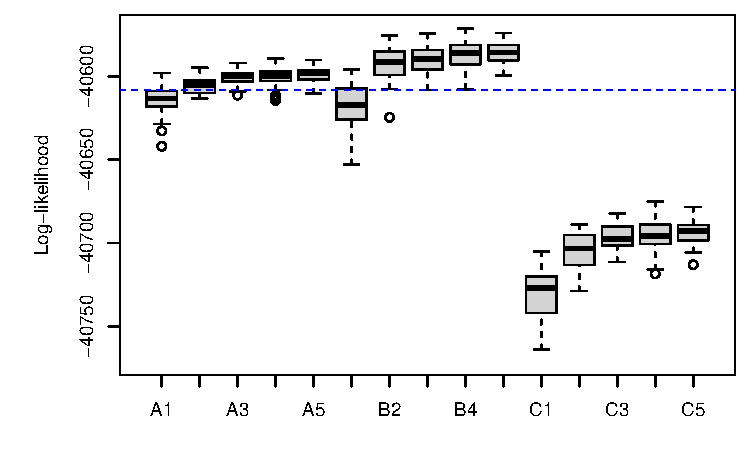
\includegraphics[width=5.5in]{figure/sim_search_boxplot-1} \hfill{}

\caption[Fitting different models to the simulated measles data, using an initial search and four further refinement searches]{Fitting different models to the simulated measles data, using an initial search and four further refinement searches. (A) $4\times 20$ unit-specific parameters and $9$ shared parameters; (B) $13\times 20$ unit-specific parameters and no shared parameters. (C) Also all unit-specific, but with immigration rather than coupling, matching the model of He et al (2010). The horizontal dashed line denotes the likelihood obtained by He et al, using \code{pomp}. Here, $J=4000$, and the random walk standard deviation (on log- and logit-transformed parameters) is 0.005 for the initial search and 0.00125 for subsequent refinements.}\label{fig:sim_search_boxplot}
\end{figure}

\end{knitrout}


\begin{knitrout}
\definecolor{shadecolor}{rgb}{1, 1, 1}\color{fgcolor}\begin{figure}

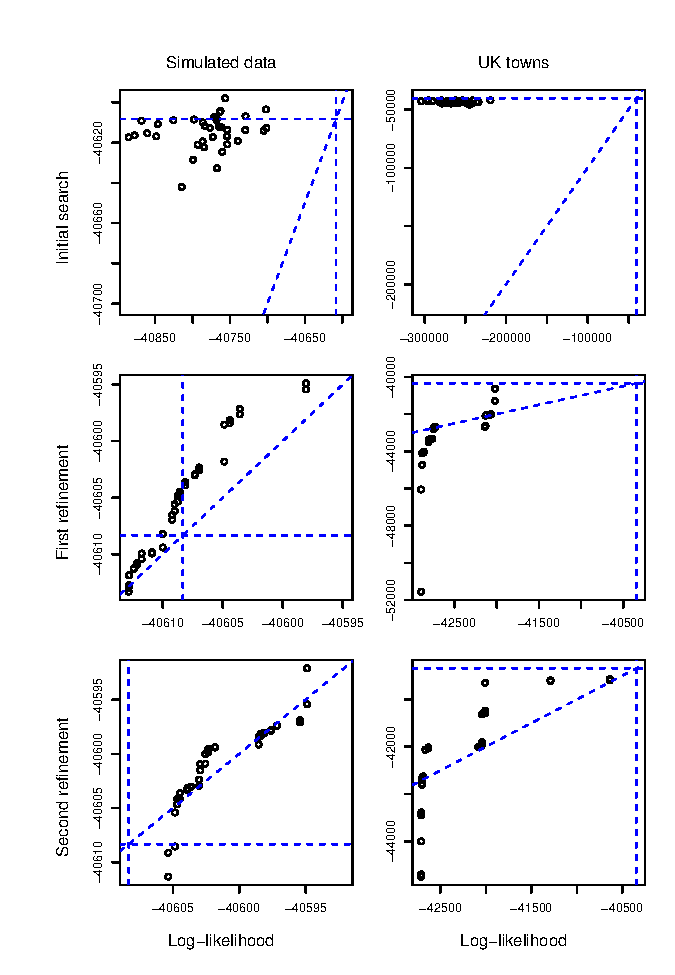
\includegraphics[width=5in]{figure/search_diagnostics-1} \hfill{}

\caption[Three steps of a likelihood search on simulated data (left panels) and UK measles data (right panels)]{Three steps of a likelihood search on simulated data (left panels) and UK measles data (right panels). Final log-likelihood values are plotted against starting log-likelihood for an initial search (top row), a refinement of this search (second row) and a second refinement (third row). Starting values for each refinement were 4 copies of the top 25\% of end points for the previous search. Unit-specific parameters were $\rho$, $S_0$, $E_0$, $I_0$ (for the simulation study, model A) and all parameters (for the data, model B).}\label{fig:search_diagnostics}
\end{figure}

\end{knitrout}


In Fig.~\ref{fig:search_diagnostics} we take a closer look at convergence diagnostics corresponding to A for the simulated data (the first column) and B for the UK measles data (the second column).
For now, we focus on the first column.
The first row plots the log-likelihood obtained after the initial search against the log-likelihood of the randomly selected starting value.
The horizontal and vertical dashed lines denote the likelihood at the truth, and the diagonal dashed line represents equality, so that points above the diagonal show improvement after the search.
We find that {\ibpf} robustly and rapidly approaches a neighborhood of the MLE, as measured by likelihood.
The second row shows that further investigation of the more successful searches can reliably obtain likelihood values higher than those at the truth.
However, for a Monte Carlo search based on Monte Carlo likelihood evaluation, it may be anticipated that pinpointing the exact maximum in a high-dimensional space is problematic.
The third row shows that continued searching does not lead to substantially better outcomes.
When using these methods, we emphasize the need to make proper inferences despite imperfect maximization \citep{ionides17,ning21}.


The results in Fig.~\ref{fig:sim_search_boxplot} and the first column of  Fig.~\ref{fig:search_diagnostics} document that {\ibpf} can be effective on simulated data, but do not guarantee comparable performance for our data analysis.
Indeed, model misspecification that is inevitable for data analysis may be expected to add difficulties to filtering and therefore to numerical methods based on filtering.
Rather, we view the simulation study as a lower bound on the effort required to carry out effective inference on data, and a starting point for investigating effective ways to proceed with the data analysis. Before moving on to the data analysis, we briefly describe the details of the model.

\subsection{The measles data and model}
\label{sec:model}

The data we consider here are weekly case reports for twenty towns, identical to those studied by \citet{he10}.
Some previous analyses have used counts aggregated over two week intervals \citep{park20,ionides21} since these were available for more cities, but our goal here is to extend the analysis of \citet{he10}.
Apart from this, our model matches \citet{ionides21} and for completeness we repeat the description here.
We compartmentalize the population of each city into susceptible ($S$), exposed ($E$), infectious ($I$), and recovered/removed ($R$) categories.
The numbers of individuals in each compartment for city $\unit$ at time $t$ are denoted by integer-valued random variables $S_\unit(t)$, $E_\unit(t)$, $I_\unit(t)$, and $R_\unit(t)$.
The population dynamics are written in terms of counting processes $N_{AB,\unit}(t)$ enumerating cumulative transitions in city $\unit$, up to time $t$, between compartments $A$ and $B$.
Here, $A,B\in \{S,E,I,R,B,D\}$ with $B$ denoting a source compartment for immigration or birth, and $D$ a sink compartment for emigration or death.
We enumerate the $U=20$ cities studied by \citet{he10} in decreasing size, so that $\unit=1$ corresponds to London.
Our model is described by the following system of stochastic differential equations, for $\unit=1,\dots, \Unit$,
\begin{equation}
\nonumber
%\label{eq:measles:system}
\begin{array}{lllllll}
\displaystyle dS_\unit(t) &=& dN_{BS,\unit}(t) &-& dN_{SE,\unit}(t) &-& dN_{SD,\unit}(t), \\
\displaystyle dE_\unit(t) &=& dN_{SE,\unit}(t) &-& dN_{EI,\unit}(t) &-& dN_{ED,\unit}(t), \\
\displaystyle dI_\unit(t) &=& dN_{EI,\unit}(t) &-& dN_{IR,\unit}(t) &-& dN_{ID,\unit}(t). 
\end{array}
\end{equation}
The total population $P_\unit(t)=S_\unit(t)+E_\unit(t)+I_\unit(t)+R_\unit(t)$ is calculated by smoothing census data and is treated as known.
The number of recovered individuals $R_\unit(t)$ in city $\unit$ is therefore defined implicitly.
$N_{SE,\unit}(t)$ is modeled as negative binomial death processes \citep{breto09,breto11}
with over-dispersion parameter $\sigma_{SE}$, and rate given by
\begin{eqnarray}
\nonumber
\mathbb{E} \big[ N_{SE,\unit}(t+dt) - N_{SE,\unit}(t) \big] 
&=& 
\beta(t) \, S_\unit(t) 
\Big[ 
  \left( \frac{I_\unit+\iota}{P_\unit} \right)^\alpha
\\
\label{eq:dEdt}
&& \hspace{-3.8cm}
 + \sum_{\altUnit \neq \unit} \frac{v_{\unit\altUnit}}{P_\unit} 
  \left\{ 
    \left(
      \frac{ I_{\altUnit} }{ P_{\altUnit} }
    \right)^\alpha - 
    \left(
      \frac{I_\unit}{P_\unit}  
    \right)^\alpha
  \right\}
\Big] dt + o(dt),\label{eqn:transmissionrate}
\end{eqnarray}
where $\beta(t)$ models seasonality driven by high contact rates between children at school, described by
\begin{equation}
\nonumber
  \beta(t)=\begin{cases}
\big(1+\amplitude(1-p)p^{-1} \big)\, \meanBeta & \mbox{ during school term},\\
\big( 1-\amplitude\big) \, \meanBeta& \mbox{ during vacation},
  \end{cases} \label{eq:term}
\end{equation}
with $p = 0.759$ being the proportion of the year taken up by the school terms, $\meanBeta$ is the mean transmission rate, and $\amplitude$ measures the reduction of transmission during school holidays.
In \eqref{eq:dEdt}, $\alpha$ is a mixing exponent modeling inhomogeneous contact rates within a city, and $\iota$ models immigration of infected individuals which is appropriate when analyzing a subset of cities that cannot be treated as a closed system.
The number of travelers from city $\unit$ to $\altUnit$ is denoted by $v_{\unit\altUnit}$. 
Here, $v_{\unit\altUnit}$ is constructed using the gravity model of \cite{xia04}, 
\[
v_{\unit\altUnit} = \gravity \cdot \frac{\;\overline{\dist}\;}{\bar{P}^2} \cdot \frac{P_\unit \cdot P_{\altUnit}}{\dist(\unit,\altUnit)},
\]
where $\dist(\unit,\altUnit)$ denotes the distance between city $\unit$ and city $\altUnit$, $P_\unit$ is the average population for city $\unit$ across time, $\bar{P}$ is the average population across cities, and $\overline{\dist}$ is the average distance between a randomly chosen pair of cities.
Here, we model $v_{\unit\altUnit}$ as fixed through time and symmetric between any two arbitrary cities, though a natural extension would allow for temporal variation and asymmetric movement between two cities.
The transition processes $N_{EI,\unit}(t)$, $N_{IR,\unit}(t)$ and $N_{\bullet D,\unit}(t)$ are modeled as conditional Poisson process with per-capita rates $\mu_{EI}$, $\mu_{IR}$ and $\mu_{\bullet D}$ respectively, and we fix $\mu_{\bullet D}=(50 \mbox{ year})^{-1}$.
The birth process $N_{BS,\unit}(t)$ is an inhomogeneous Poisson processes with rate $\mu_{BS,\unit}(t)$, given by interpolated census data.

To describe the measurement process, let $Z_{\unit\comma\time}=N_{IR\comma\unit}(t_\time)-N_{IR\comma\unit}(t_{\time-1})$ be the number of removed infected individuals in the $n$th reporting interval.
Suppose that cases are quarantined once they are identified, so that reported cases comprise a fraction $\rho$ of these removal events.
The case report $\data{y}_{\unit\comma\time}$ is modeled as a realization of a discretized conditionally Gaussian random variable $Y_{\unit\comma\time}$, defined for $y>0$ via
\begin{eqnarray}
\nonumber
\prob\big[Y_{\unit\comma\time}{=}y\mid Z_{\unit\comma\time}{=}z\big] &=& \Phi\big(y+0.5; \rho z,\rho(1-\rho)z+\psi^2\rho^2z^2\big)
\\
&&\hspace{-20mm}
- \Phi\big(y-0.5; \rho z,\rho(1-\rho)z+\psi^2\rho^2z^2\big)
\label{eq:obs}
\end{eqnarray}
where $\Phi(\cdot;\mu,\sigma^2)$ is the $\normal(\mu,\sigma^2)$ cumulative distribution function, and $\psi$ models overdispersion relative to the binomial distribution.
For $y=0$, we replace $y-0.5$ by $-\infty$ in \eqref{eq:obs}.

Three data points were treated as missing by \citet{he10} due to presumed recording errors, and we followed that decision.
The general SpatPOMP framework has flexibility that permits modeling of missing data in various ways. 
We chose to include a special value $\mathrm{NA}$ in $\Yspace$ and set $Y_{u,n}$ to be $\mathrm{NA}$ with probability one when $\data{y}_{u,n}$ is missing.

\section{Demonstration on data}
\label{sec:data}

\begin{knitrout}
\definecolor{shadecolor}{rgb}{1, 1, 1}\color{fgcolor}\begin{figure}

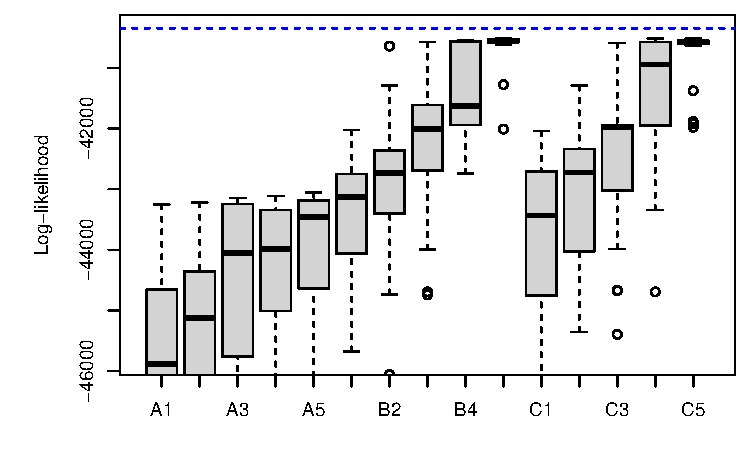
\includegraphics[width=5.5in]{figure/data_search_boxplot-1} \hfill{}

\caption[Fitting different models to the UK measles data using the method tested on simulated data]{Fitting different models to the UK measles data using the method tested on simulated data. (A) $4\times 20$ unit-specific parameters and $9$ shared parameters; (B) $13\times 20$ unit-specific parameters and no shared parameters. (C) Also all unit-specific, but with immigration rather than coupling, matching the model of He et al (2010). The horizontal dashed line denotes the likelihood obtained by He et al, using \code{pomp}.}\label{fig:data_search_boxplot}
\end{figure}

\end{knitrout}


Fig.~\ref{fig:data_search_boxplot} shows results for fitting models A, B and C to UK measles data using successive rounds of {\ibpf}, applying the same method used for the simulation study shown in Fig.~\ref{fig:sim_search_boxplot}.
The dashed lines show the sum of the log-likelihoods obtained by \citet{he10}, $\ell_{\mathrm He}=-40345.7$.
The value $\ell_{\mathrm He}$ corresponds to model C.
BPF with each town forming a separate block, applied to an uncoupled model such as C, is equivalent to carrying out independent particle filters for each unit.
Indeed, if the published parameter values from \citet{he10} are inserted into the \code{spatPomp} object for model C, then the \code{bpfilter()} function can be used to carry out BPF, which retrieves $\ell_{\mathrm He}$, up to Monte Carlo error.
Each of models A, B and C in Fig.~\ref{fig:data_search_boxplot} shows shortfall relative to $\ell_{\mathrm He}$.

The largest shortfall is for A, and an explanation is that A has more shared parameters than the evidence in the data supports.
The results of \citet{he10} suggest that the data are explained better when various parameters are a function of the town population.
However, it remains an open problem to determine suitable functional forms for this relationship, and to establish regularities across towns that can be represented by shared parameters.
This may be investigated using panel methods such as PanelPOMP models \citep{breto19} in addition to consideration of SpatPOMP models.

Models B and C give rise to comparable likelihoods, which is in contrast to Fig.~\ref{fig:sim_search_boxplot}.
Fitting to simulated data from B (in the special case where all unit-specific parameters are equal across all units) the shortfall for C in Fig.~\ref{fig:sim_search_boxplot} indicates that we obtain a substantially worse fit by approximating coupling by an uncoupled reservoir of infection.
If the actual data were also explained substantially better by a coupled model, we would expect to see comparable results in the data analysis.
Since we do not, we conclude that this coupled model is not a substantially better explanation than the uncoupled model.
Various other candidate coupling mechanisms have been proposed \citep{bjornstad19} but they have not yet been fitted to the full data, suggesting a lack of appropriate methodology to do so.
Instead, \citet{bjornstad19} looked at summary statistics based on local fade-outs and re-introductions.
Further investigation is needed to determine whether other models for coupling can show improvement over this gravity model on these data.
This should be carried out in conjunction with research into the specification of shared and unit-specific parameters.

We notice from Fig.~\ref{fig:data_search_boxplot} that model B has a small but distinct shortfall compared to $\ell_{\mathrm He}$.
On the simulated data, we do not observe this shortfall, and we deduce that the real data provides a more challenging optimization environment.
When carrying out hard optimization problems, it may be possible to develop helpful strategies specific to the model and data in question.
For example, one could try merging unit-specific parameters from different searches, using the likelihood component for each unit to assess successful choices.
Optimization heuristics such as this do not have general theoretical support; if they obtain higher likelihoods that is sufficient justification. 
For analysis of panel time series data using PanelPOMP models, such methods have clearer theoretical support and have been found useful \citep{breto19}.

\section{Discussion}
\label{sec:discussion}

Theoretical interest in BPF was inspired by \citet{rebeschini15} who showed mathematically that BPF can, under particular conditions, enjoy linear scaling properties.
\citet{rebeschini15} expressed pessimism about the practical applicability of their algorithm, which may help to explain why the practical use of this algorithm has been limited.
The algorithm was independently invented under the name of a factored particle filter by \citet{ng02} who offered an empirical justification.
However, the proposal of \citet{ng02} also saw only limited use.
The numerical results in Fig.~3 of \citet{ionides21} suggest that BPF is particularly well suited to metapopulation models.
In a metapopulation model, one expects most of the population dynamics to occur at a local level, among the individuals at one spatial unit.
As a broad generalization, in ecological systems dispersion of individuals between spatial units is rare but dynamically important.
Edge effects between blocks, which may be a serious problem for BPF in a system with stronger spatial coupling \citep{ionides21} can therefore be a relatively minor concern for metapopulation models.
Blocks of size one unit are therefore a natural choice for block filtering of metapopulation models when the constituent populations are spatially distinct.

This article has investigated a likelihood maximization approach to inference.
Much research has been done on inference for high-dimensional partially observed stochastic dynamic systems, and we have cited above only the most directly relevant work.
A Bayesian inference approach based on the ensemble Kalman filter was developed by \citet{katzfuss19}.
An expectation-maximization approach based on a block particle filter was presented by \citet{finke17}.
Spatiotemporal models having a convenient factorization across units were studied by \citet{beskos17} and \citet{xu19}.

Computation time for Fig.~\ref{fig:sim_search_boxplot} and Fig.~\ref{fig:data_search_boxplot} was approximately 24hr on a single core of a compute node for 4000 particles iterated 100 times over the 730 time points (weekly data for 14 years) for 20 cities.
Each box in these figures involves 36 replications and thus took 24hr on all cores of one node on a computing cluster.
This level of effort is tolerable, but does suggest that the methods will not readily extend to tasks that are considerably larger. 
In particular, we do not expect applicability to situations where it is necessary to consider $10^3$ or more spatial units.
In such situations, it may be necessary to make additional approximations such as those inherent in the ensemble Kalman filter \citep{evensen09,katzfuss19} or other numerical filtering techniques \citep{whitehouse22}.
However, we anticipate that many practical metapopulation analyses can be addressed within the scope we have demonstrated.
The majority of the computational effort is spent on simulating from the dynamic model.
In the \code{spatPomp} R package, as in \code{pomp}, the user supplies a snippet of C code for simulating a single particle between a single arbitrary pair of times, and the package provides a vectorized form of this computation which is used by the inference methodologies within the package.
As a consequence, competitive computational performance is obtained even though the majority of the package is written in R \citep[Table~1]{FitzJohn20}.

\vspace{3mm}

%\newpage

\noindent {\bf Code and data availability}

\vspace{1mm}

\noindent The data we analyze are in the public domain, and are available together with source code at \url{https://github.com:ionides/ibpf_article}.

\vspace{3mm}

\noindent {\bf Acknowledgments}

\vspace{1mm}

\noindent This work was supported by National Science Foundation grants DMS-1761603 and DMS-1646108, and National Institutes of Health grant 1-R01-AI143852. We acknowledge an anonymous referee from a previous article who recommended that we should try implementing a block particle filter.

\bibliography{bib-ibpf}

% \vspace{8mm}
\newpage

\noindent{\bf \Large Appendix A}

\vspace{3mm}

\noindent{\bf \large Varying the IBPF spatial autoregression parameter, $\spatReg$}

\vspace{-5mm}

\begin{knitrout}
\definecolor{shadecolor}{rgb}{1, 1, 1}\color{fgcolor}\begin{figure}[h]

\includegraphics[width=5.5in]{figure/spatreg_boxplot-1} \hfill{}

\caption[Varying the spatial autoregression algorithmic parameter for shared parameters with simulated measles data]{Varying the spatial autoregression algorithmic parameter for shared parameters with simulated measles data. The log-likelihood was obtained using $M=100$ iterations of IBPF starting at random parameters (median starting log-likelihood, -40800). The horizontal dashed line denotes the log-likelihood at the true parameters}\label{fig:spatreg_boxplot}
\end{figure}

\end{knitrout}

\end{document}
